\documentclass[11pt, oneside]{article}   	% use "amsart" instead of "article" for AMSLaTeX format
\usepackage{geometry}                		% See geometry.pdf to learn the layout options. There are lots.
\geometry{letterpaper}                   		% ... or a4paper or a5paper or ... 
\usepackage{graphicx}				% Use pdf, png, jpg, or eps§ with pdflatex; use eps in DVI mode
								% TeX will automatically convert eps --> pdf in pdflatex		
\usepackage{amssymb}
\usepackage{amsmath}
\usepackage{parskip}
\usepackage{color}
\usepackage{hyperref}

\graphicspath{{/Users/telliott_admin/Dropbox/Tex/png/}}
% \begin{center} 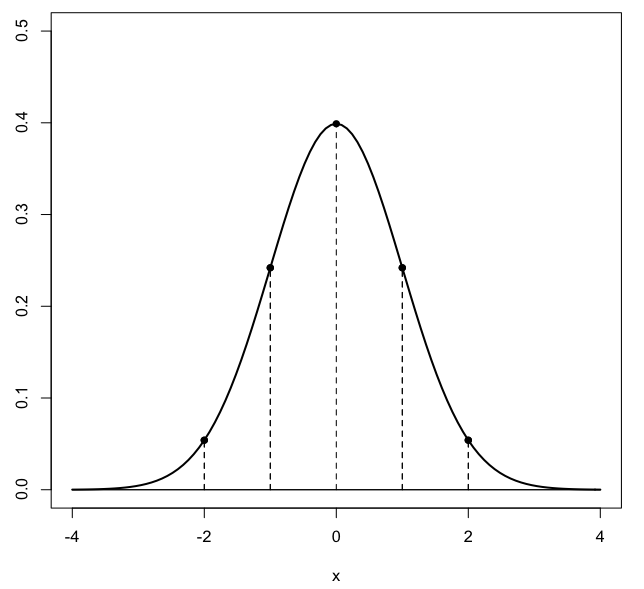
\includegraphics [scale=0.4] {gauss3.png} \end{center}

%break
\title{Vector rotation}
\date{}

\begin{document}
\maketitle
\Large
If you know something about matrix multiplication, just remember this result:
\[
\begin{bmatrix}  x' \\ y' \end{bmatrix}
=
\begin{bmatrix}  
\cos \theta & -\sin \theta \\
\sin \theta & \ \  \cos \theta 
\end{bmatrix}
\begin{bmatrix}  x \\ y \end{bmatrix}
\]

If not, read on.

Our goal here is to find the equations for rotation of coordinates.  We want to be as simple as we can, so that we can remember how the derivation works.  We will need a couple of preliminary facts, however.

\begin{itemize}
\item a procedure to compute the dot product of two vectors
\item two vectors are $\perp$ (orthogonal) $\iff$ the dot product is zero
\item the projection of a vector $\mathbf{a}$ onto \emph{any} other \textbf{unit} vector $\mathbf{\hat{e}}$ is just the dot product $\mathbf{a} \cdot \mathbf{\hat{e}}$ 
\item a rotated set of coordinates is a set of orthogonal unit vectors (in whatever direction we choose)
\end{itemize}

Recall that the dot product is a number computed from the components of any two vectors $\mathbf{a}$ and $\mathbf{b}$ by the following procedure:
\[ \mathbf{a} \cdot \mathbf{b} = a_1 b_1 + a_2 b_2 + \dots + a_n b_n \]

Some examples:
\[ \langle 3, 2 \rangle \cdot  \langle 2, 5 \rangle = 3 \times 2 + 2 \times 5 = 16 \]
\[ \langle 1, 0 \rangle \cdot  \langle 0, 1 \rangle = 0 \]
\[ \langle \cos \theta, \sin \theta \rangle \cdot  \langle -\sin \theta, \cos \theta \rangle = 0 \]

As we might expect, the unit vector along the $x$-axis, usually called $\hat{\mathbf{i}}$, and the unit vector along the $y$-axis, $\hat{\mathbf{j}}$, are perpendicular to each other (second example, above).

Similarly, for any angle $\theta$, the given vectors $\langle \cos \theta, \sin \theta \rangle$ and $\langle -\sin \theta, \cos \theta \rangle$ are perpendicular.  These two examples should suggest to you a general method for finding a second vector orthogonal to one you are given.

The length of a vector $\mathbf{a}$ is represented as $|\mathbf{a}|$, or even just $a$, and the length squared is

\[ a^2 = \mathbf{a} \cdot \mathbf{a} \]

With respect to the projection, an example should also make that clearer.  Suppose we are working with two-dimensional vectors and we decide that our new $x$-axis should be in the direction of the vector $3,4$.  The first thing to do is to re-scale this to be a unit vector.  The length squared is
\[ \langle 3, 4 \rangle \cdot  \langle 3, 4 \rangle = 9 + 16 = 25 \]

Hence the length is $5$ and our new unit vector $\mathbf{\hat{u}}$ is 
\[ \mathbf{\hat{u}} = \langle 3/5, 4/5 \rangle \]

We also need a unit vector $\mathbf{\hat{v}}$ such that $\mathbf{\hat{u}} \cdot \mathbf{\hat{v}} = 0$.  We obtain
\[ \mathbf{\hat{v}} = \langle -4/5, 3/5 \rangle \]
or 
\[ \mathbf{\hat{v}} = \langle 4/5, -3/5 \rangle \]
These two vectors are the same vector, just pointing in opposite directions (which is in the same direction, for the purpose of vectors).

Then for \emph{any} vector $\mathbf{a}$, we can compute the same vector in a set of rotated coordinates based on $\mathbf{u}$ and $\mathbf{v}$ as
\[ a_u = \mathbf{a} \cdot \mathbf{\hat{u}} \]
\[ a_v = \mathbf{a} \cdot \mathbf{\hat{v}} \]

\subsection*{derivation}

All we have to do is to think about rotation of the unit vectors $\hat{\mathbf{i}}$ and $\hat{\mathbf{j}}$ through an angle $\theta$ counter-clockwise.  

Start with $\hat{\mathbf{i}}$.  The new vector we seek is still a unit vector, but rotated so that it forms an angle $\theta$ with the positive $x$-axis.

The new vector has both $\hat{\mathbf{i}}$ and $\hat{\mathbf{j}}$ components. Projection onto $\hat{\mathbf{i}}$ gives a vector with unit length times $\cos \theta$ or just $\cos \theta$, and similarly, the projection onto $\hat{\mathbf{j}}$ gives a length $\sin \theta$.  Clearly the squared length is $\cos^2 \theta + \sin^2 \theta$, so this is a unit vector.

In vector notation we would say that
\[ \langle 1,0 \rangle \ \Rightarrow \ \langle \cos \theta, \sin \theta \rangle \]
In matrix language the two vectors are related in this way:
\[
\begin{bmatrix}  
1  \\  
0  
\end{bmatrix}
\Rightarrow
\begin{bmatrix}  
\cos\  \theta  \\  
\sin\  \theta  
\end{bmatrix}
\]
where $\Rightarrow$ refers to rotation.

So the question is, what matrix will multiply $\hat{\mathbf{i}}$ to give this result?
\[
\begin{bmatrix}  
a & b  \\  
c & d  
\end{bmatrix}
\begin{bmatrix}  
1  \\  
0  
\end{bmatrix}
=
\begin{bmatrix}  
\cos\  \theta  \\  
\sin\  \theta  
\end{bmatrix}
\]
Recall that matrix multiplication works like this
\begin{center} 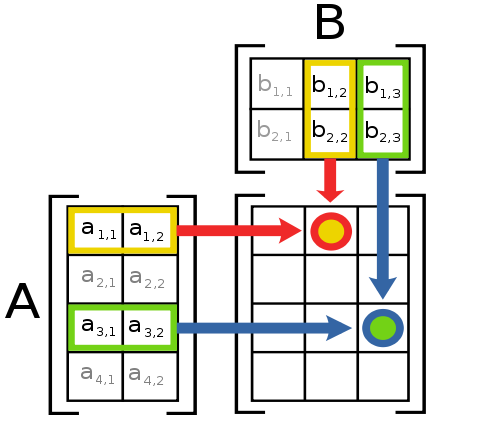
\includegraphics [scale=0.35] {mm1.png} \end{center}

For a matrix times a vector, $B$ would have only a single column.

So going back to this:

\[
\begin{bmatrix}  
a & b  \\  
c & d  
\end{bmatrix}
\begin{bmatrix}  
1  \\  
0  
\end{bmatrix}
=
\begin{bmatrix}  
\cos\  \theta  \\  
\sin\  \theta  
\end{bmatrix}
\]


I hope it's pretty clear that $a = \cos \theta$ and $c = \sin \theta$:
\[
\begin{bmatrix}  
\cos \theta & b  \\  
\sin \theta & d  
\end{bmatrix}
\begin{bmatrix}  
1  \\  
0  
\end{bmatrix}
=
\begin{bmatrix}  
\cos\  \theta  \\  
\sin\  \theta  
\end{bmatrix}
\]
Can you see why this is true?

On the other hand, rotation of the unit $\hat{\mathbf{j}}$ vector by $\theta$ should give
\[
\begin{bmatrix}  
a & b  \\  
c & d  
\end{bmatrix}
\begin{bmatrix}  
0  \\  
1  
\end{bmatrix}
=
\begin{bmatrix}  
-\sin \  \theta  \\  
\ \ \cos \  \theta  
\end{bmatrix}
\]
The minus sign comes because the new unit vector is now sticking out into the second quadrant.

Again, it should be clear that 
\[
\begin{bmatrix}  
a & -\sin \  \theta  \\  
c & \ \ \cos \  \theta  
\end{bmatrix}
\begin{bmatrix}  
0  \\  
1  
\end{bmatrix}
=
\begin{bmatrix}  
-\sin \  \theta  \\  
\ \ \cos \  \theta  
\end{bmatrix}
\]

Now, just put them together:
\[
R_{ccw} = 
\begin{bmatrix}   \ \cos \theta & -\sin \theta  \\  \ \sin \theta & \ \ \cos \theta  \end{bmatrix}
\]
\[
\begin{bmatrix}   \ \cos \theta & -\sin \theta  \\  \ \sin \theta & \ \ \cos \theta  \end{bmatrix}
\begin{bmatrix}   x   \\  y  \end{bmatrix} = \begin{bmatrix}   u   \\  v  \end{bmatrix}
\]
In particular, a rotation of $90^{\circ}$ ccw goes like this
\[
\begin{bmatrix}   0 & -1  \\  1 & \ \ 0  \end{bmatrix}
\begin{bmatrix}   1   \\  0  \end{bmatrix} = \begin{bmatrix}   0   \\  1  \end{bmatrix}
\]
$\hat{\mathbf{i}}$ is rotated to become $\hat{\mathbf{j}}$.

\[
\begin{bmatrix}   0 & -1  \\  1 & \ \ 0  \end{bmatrix}
\begin{bmatrix}   0   \\  1  \end{bmatrix} = \begin{bmatrix}   -1   \\  0  \end{bmatrix}
\]
$\hat{\mathbf{j}}$ is rotated to become $-\hat{\mathbf{i}}$.

I claim that since the matrix we found works for both of the unit vectors it will work for any vector, since any vector can be written as a linear combination of the unit vectors
\[ \mathbf{a} = a_1 \ \hat{\mathbf{i}} + a_2 \ \hat{\mathbf{j}} \]

The inverse of the matrix we derived would be used for clockwise rotation and it is just
\[
R_{cw} =
\begin{bmatrix}   \ \ \ \cos \theta & \ \sin \theta  \\  -\sin \theta & \ \ \cos \theta  \end{bmatrix}
\]
You can verify this by remembering the rule for $2 \times 2$ or by multiplication
\[
R_{cw} \  R_{ccw} =
\begin{bmatrix}   \ \ \ \cos \theta & \ \sin \theta  \\  -\sin \theta & \ \ \cos \theta  \end{bmatrix}
\begin{bmatrix}   \ \cos \theta & -\sin \theta  \\  \ \sin \theta & \ \ \cos \theta  \end{bmatrix}
= 
\begin{bmatrix}   1 & 0  \\  0 & 1 \end{bmatrix}
= I
\]
Don't be confused when someone talks about rotation of the coordinate system.  Here, the coordinate system stayed fixed but we rotated the vector counter-clockwise.  We achieve the same thing (and use the same equation) for a \emph{clockwise} rotation of the coordinate system through an angle $\theta$.

\begin{center} 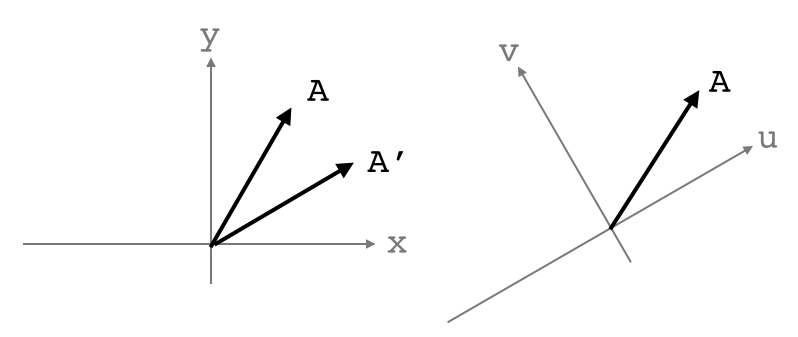
\includegraphics [scale=0.4] {rotate_vec_coord.png} \end{center}

If you really want to rotate the coordinate system counter-clockwise, rotate the vector clockwise.

\subsection*{consequence}

One other neat thing comes out of this when we ask about rotation by an angle $s + t$.  We can write two equivalent expressions, one by substituting $\theta=s+t$, and the other by doing two sequential applications of the matrix.  That is:
\[
\begin{bmatrix}   \ \cos (s+t) & -\sin (s+t)  \\  \ \sin (s+t) & \ \ \cos (s+t)  \end{bmatrix} =
\begin{bmatrix}   \ \cos s & -\sin s  \\  \ \sin s & \ \ \cos s  \end{bmatrix}
\begin{bmatrix}   \ \cos t & -\sin t  \\  \ \sin t & \ \ \cos t  \end{bmatrix}
\]
Look at the term on the upper-left, $\cos(s+t)$.  Sound familiar?  Carry out the matrix multiplication on the right for that element
\[ \cos(s+t) = \cos s \cos t - \sin s \sin t \]
We have derived the cosine addition formula.  Similarly, the bottom-left term is for the sine
\[ \sin(s+t) = \sin s \cos t + \cos s \sin t \]

\subsection*{yet another way}
We can look at this in still a different way.  Write
\[
\begin{bmatrix}  x \\ y \end{bmatrix}
=
x
\begin{bmatrix}  1 \\ 0 \end{bmatrix}
+
y
\begin{bmatrix}  0 \\ 1 \end{bmatrix}
\]
In this representation, the vector $\langle x,y \rangle$ is a linear combination of the unit vectors $\mathbf{\hat{i}} =\ \langle 1,0 \rangle$ and $\mathbf{\hat{j}}  =\ \langle 0,1 \rangle$.

To rotate the point, we just want to use a different set of unit vectors.  The new unit vectors (for the rotated axes) are $\langle \cos \theta,\sin \theta \rangle$ and $\langle -\sin \theta,\cos \theta \rangle$.  

If you compute their lengths, it is clear that they are, in fact, unit vectors.
\[
\begin{bmatrix}  x' \\ y' \end{bmatrix}
=
x
\begin{bmatrix}  \cos \theta \\ \sin \theta \end{bmatrix}
+
y
\begin{bmatrix}  -\sin \theta \\ \ \ \cos \theta \end{bmatrix}
\]
Written as a matrix multiplication, this is
\[
\begin{bmatrix}  x' \\ y' \end{bmatrix}
=
\begin{bmatrix}  
\cos \theta & -\sin \theta \\
\sin \theta & \ \  \cos \theta 
\end{bmatrix}
\begin{bmatrix}  x \\ y \end{bmatrix}
\]




\end{document}